\documentclass[11pt,a4paper,titlepage]{article}
\usepackage[utf8]{inputenc}
\usepackage[dutch]{babel}
\usepackage{amsmath}
\usepackage{amsfonts}
\usepackage{amssymb}
\usepackage{graphicx}
\usepackage{hyperref}
\usepackage{algorithm}
\usepackage{algpseudocode}\usepackage{float}
\usepackage{fullpage}
\renewcommand{\familydefault}{\sfdefault}

\algblockdefx{ForEach}{EndForEach}[2]{\textbf{for each} #1 \textbf{in} #2 \textbf{do}}{\textbf{end for}}

\author{Pieter-Jan Coenen en Stijn Caerts}
\title{Practicum Toepassingen van Meetkunde in de Informatica \\ Snijdende rechthoeken}
\date{20 mei 2016}

\begin{document}
	\maketitle
	\tableofcontents
	\newpage
	\section{Beschrijving algoritmen}
	In onze algoritmen hebben we proberen rekening te houden met de meeste rand gevallen. Als twee zijden volledig of gedeeltelijk samenvallen dan geven we als intersectie punten voor deze zijden steeds het begin punt en het eind punt, van waar tot waar ze samen vallen.  Als twee rechthoeken volledig samenvallen dan geven we als intersectie punten de vier hoekpunten van de rechthoeken.\\ \\
	Wanneer we het in de algoritme hebben over het "bereken van de snijpunten tussen twee rechthoeken" dan doen we dit steeds via de procedure vermeld in punt 2.2.1.
	\subsection{Algoritme 1}
	\emph{Algoritme 1} is een brute-force algoritme. Elke rechthoek wordt gecontroleerd met elke andere rechthoek voor snijding. Om te vermijden dat we twee rechthoeken dubbel controleren op snijpunten, houden we een hashset bij van de rechthoeken waarvoor we de snijpunten met alle andere rechthoeken al zijn nagegaan. We gebruiken een hashset omdat we dan in  $\mathcal{O}(1)$ tijd kunnen controleren of een bepaalde rechthoek al werd gecontroleerd op snijding met alle andere rechthoeken.\\ Hieronder het algoritme in pseudocode.
	\begin{algorithm}[H]
		\caption{}
		\begin{algorithmic}[1]
			\State intersections $\gets \varnothing $
			\State checked $\gets \varnothing $
			\ForEach {rect1} {rectangles}
				\ForEach {rect2} {rectangles}
					\If {rect1 $\neq$ rect2 \textit{and} rect2 $\notin$ checked}
						\State intersections $ \gets $ intersections $ \cup $ calculateIntersections(rect1, rect2)
					\EndIf
				\EndForEach
				\State checked $\gets$ checked $\cup$ rect1
			\EndForEach
		\end{algorithmic}
	\end{algorithm}
	Aangezien we twee geneste lussen hebben, en we niet dubbel controleren voor eenzelfde paar rechthoeken. De functie \emph{calculateIntersections()} wordt daarom $ (n-1) + (n-2) + \dots + 2 + 1 = \frac{n(n-1)}{2} $ keer uitgevoerd en dus heeft \emph{Algoritme 1} een complexiteit van $\mathcal{O}(n^2)$.
	
	\subsection{Algoritme 2}
	\emph{Algoritme 2} is een doorlooplijn-algoritme. Dit betekent dat we de rechthoeken gaan ordenen volgens x-coördinaat en vervolgens deze lijst met rechthoeken doorlopen. De doorlooplijn gaat volgens stijgende x-waarde en als de doorlooplijn een rechthoek snijdt, voegen we die rechthoek toe aan de lijst van actieve rechthoeken. Als de rechthoek niet langer gesneden wordt door de doorlooplijn, verwijderen we de rechthoek weer uit de lijst van actieve rechthoeken. Als we een nieuwe rechthoek tegenkomen, controleren we enkel of er snijding is tussen die rechthoek en de rechthoeken die op dat moment actief zijn. Dit zorgt er voor dat we meestal minder vaak moeten controleren of twee rechthoeken snijden. In de worst case moeten we bij dit algoritme echter ook voor alle andere rechthoeken controleren of er snijding optreedt. Dit is het geval als alle rechthoeken samen actief is.
	\begin{algorithm}[H]
		\caption{}
		\begin{algorithmic}[1]
			\State intersections $\gets \varnothing $
			\State queue $\gets$ priority queue van rechthoeken gesorteerd op de x-coördinaat, initieel van het punt linksonder.
			\State active $\gets \varnothing$
			\While {queue is not empty}
				\State rect1 = queue.poll()
				\If {rect $\notin$ active}
					\State voeg rect toe aan de queue, met de x-coordinaat van het punt rechtsboven als sorteringscriterium.
					\State snijpunten $\gets$ snijpunten $\cup$ alle snijpunten van rect met alle andere rechthoeken die actief zijn
					\State active $\gets$ active $\cup$ rect
				\Else
					\State active $\gets$ active $\backslash$ rect
				\EndIf
			\EndWhile
		\end{algorithmic}
	\end{algorithm}
	
	\subsection{Algoritme 3}
	\emph{Algoritme 3} is gebaseerd op \emph{algoritme 2}, het werkt grotendeels op dezelfde manier. Maar in plaats van de actieve rechthoeken te bewaren in een array, bewaren we ze deze keer in Red-Black Tree. Op deze manier kunnen we veel efficiënter gaan controleren op snijding. We voegen namelijk elke rechthoek die actief wordt twee keer toe aan deze Red-Black Tree, een keer met zijn grootste y-coördinaat als key en een keer met zijn kleinste y-coördinaat als key.  Wanneer we vervolgens gaan controleren op snijding van een bepaalde driehoek met de andere actieve rechthoeken dan kunnen we direct gaan kijken naar de rechthoeken die minstens één horizontale zijde hebben die tussen de minimale en de maximale y-coördinaat ligt van de desbetreffende rechthoek. Op deze manier vinden we onmiddellijk alle rechthoeken waarmee er wordt gesneden zonder dat we de volledige lijst van actieve rechthoeken moeten doorlopen (tenzij de desbetreffende rechthoek natuurlijk snijdt met alle actieve rechthoeken). Nog een verschil met algoritme twee is dat we nu niet enkel moeten gaan controleren op snijding wanneer we een element toevoegen, maar ook wanneer we een rechthoek terug verwijderen uit de actieve queue. Dit is omdat op het moment van verwijderen er eventueel nieuwe rechthoeken zijn toegevoegd, die kleiner zijn dan de betreffende rechthoek waardoor bij het toevoegen van die rechthoek de snijding nog niet wordt gedetecteerd.  Daarom moeten we opnieuw controleren op snijding bij het verwijderen van een rechthoek. \\ \\
	We hebben in onze implementatie gekozen voor een Red-Black Tree, omdat dit de meest efficiënte manier is om een rij gesorteerd te houden en er in  $\mathcal{O}(\log n)$ tijd elementen aan toe te voegen en uit te verwijderen.	
		\begin{algorithm}[H]
			\caption{}
			\begin{algorithmic}[1]
				\State intersections $\gets \varnothing $
				\State queue $\gets$ priority queue van rechthoeken gesorteerd op de x-coördinaat van het punt linksonder.
				\State active $\gets \varnothing$
				\While {queue is not empty}
				\State rect1 = queue.poll()
				\If {rect $\notin$ active}
				\State voeg rect toe aan de queue, met de x-coordinaat van het punt rechtsboven als sorteringscriterium.
				\State snijpunten $\gets$ snijpunten $\cup$ alle snijpunten van rect met alle andere rechthoeken die actief zijn en waarvan de ondersten en/of bovenste zijde van die rechthoeken zich bevindt tussen de kleinste en grootste y-coördinaat van rect.
				\State active $\gets$ active $\cup$ twee keer rect toevoegen, één keer met zijn grootste y-coördinaat als sorteringscriterium en nog een keer met zijn kleinste y-coördinaat als sorteringscriterium.
				\Else
				\State active $\gets$ active $\backslash$ alle voorkomens van rect
				\State snijpunten $\gets$ snijpunten $\cup$ alle snijpunten van rect met alle andere rechthoeken die actief zijn en waarvan de ondersten en/of bovenste zijde van die rechthoeken zich bevindt tussen de kleinste en grootste y-coördinaat van rect.
				\EndIf
				\EndWhile
			\end{algorithmic}
		\end{algorithm}
	
	\section{Experimenten en correctheid}
		\subsection{Experimenten}
		We hebben verschillende experimenten uitgevoerd om de complexiteit van onze algoritmes na te gaan. Eerste hebben we een doubeling experiment uitgevoerd waarbij de x- en y-coördinaten van de hoekpunten tussen 0 en 1 liggen.  Nadien hebben opnieuw verschillende doubeling experimenten uitgevoerd waarbij de lengte van de zijdes van de rechthoeken tussen  respectievelijk 0 en 0.01, 0.01, 0.2 en 0.5 lagen.\\ We hebben een doubeling experiment gebruikt om dat dit volgens ons de ideale methode is om analyseren hoe de algoritmes zich gedragen naarmate de invoer groter wordt. De interpretatie van de resultaten bespreken we later in puntje 3.
			\subsubsection{Doubeling experiment met hoekpunten tussen 0 en 1}
				We hebben een doubeling experiment uitgevoerd waarbij het aantal rechthoeken laten toenemen vanaf 1 tot 8192.  We hebben hierbij de tijd in miliseconden gemeten die de drie algoritme nodig hebben om de snijpunten van de rechthoeken te vinden.
				\begin{figure}[H]
				\centering
				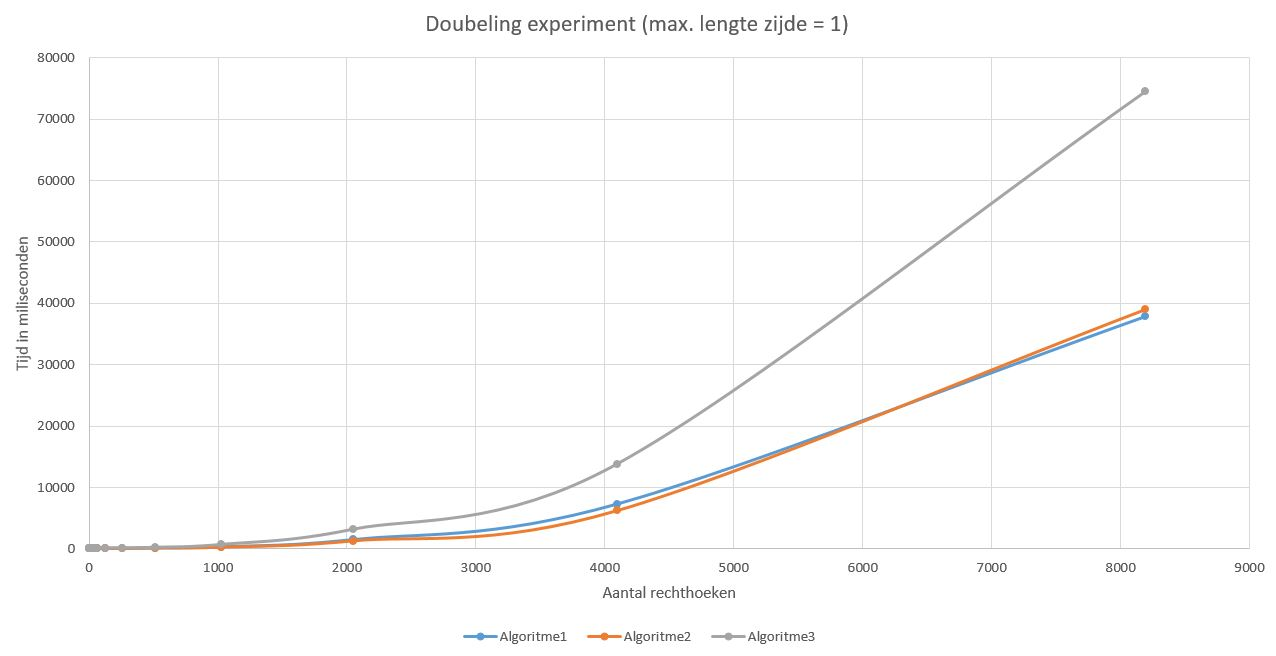
\includegraphics[width=0.75\textwidth]{zijde1.JPG}
				\caption{\label{fig:convR}Grafiek voor het doubeling experiment met zijde die variëren tussen 0 en 1}
				\end{figure}
			\subsubsection{Doubeling experiment voor verschillende lengtes van de zijden}
				Ook hier hebben we een doubeling experiment uitgevoerd.  We hebben hierbij de tijd in miliseconden gemeten die de drie algoritme nodig hebben om de snijpunten van de rechthoeken te vinden. We hebben dit experiment eerst gedaan voor zijdes met een maximale lengte van 0.01, dan voor zijdes met een maximale lengte van 0.1, vervolgens voor zijdes met een maximale lengte van 0.2 en tot slot voor zijdes met een maximale lengte van 0.5.\\ \\
				We verkregen de volgende grafieken:
				\begin{figure}[H]
				\centering
				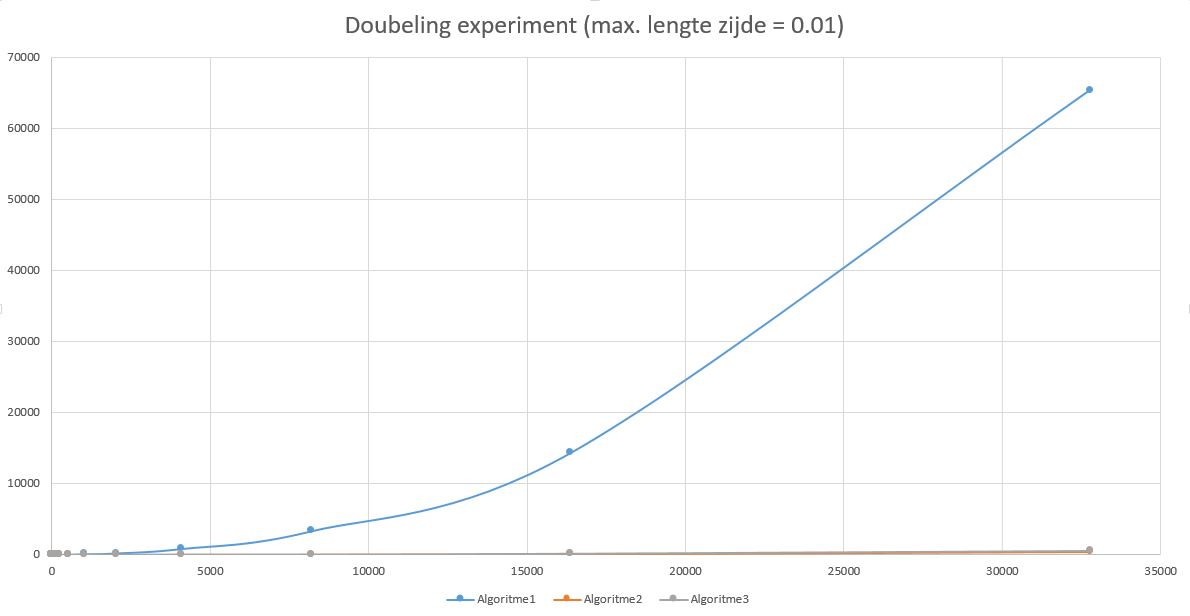
\includegraphics[width=0.75\textwidth]{zijde001.JPG}
				\caption{\label{fig:convR}Grafiek voor het doubeling experiment met zijdes die variëren tussen 0 en 0.01}
				\end{figure}
				\begin{figure}[H]
				\centering
				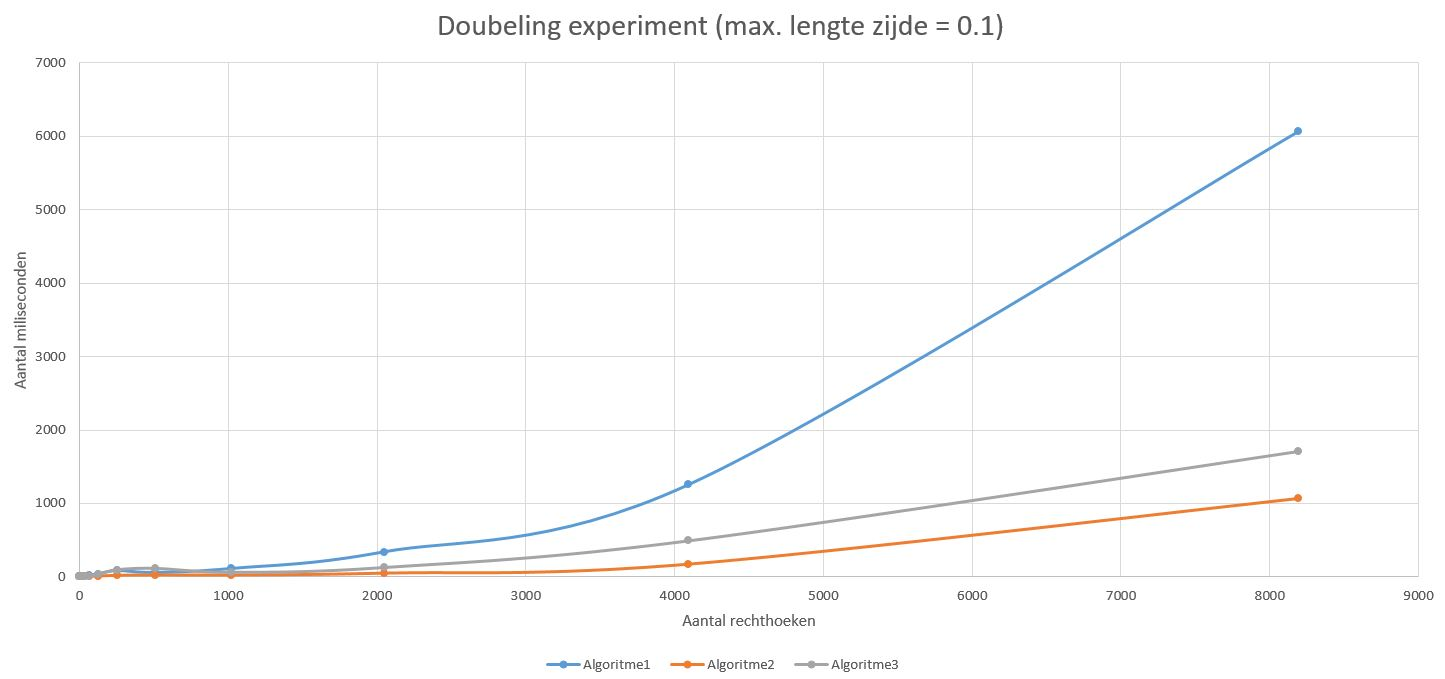
\includegraphics[width=0.75\textwidth]{zijde01.JPG}
				\caption{\label{fig:convR}Grafiek voor het doubeling experiment met zijdes die variëren tussen 0 en 0.1}
				\end{figure}
				\begin{figure}[H]
				\centering
				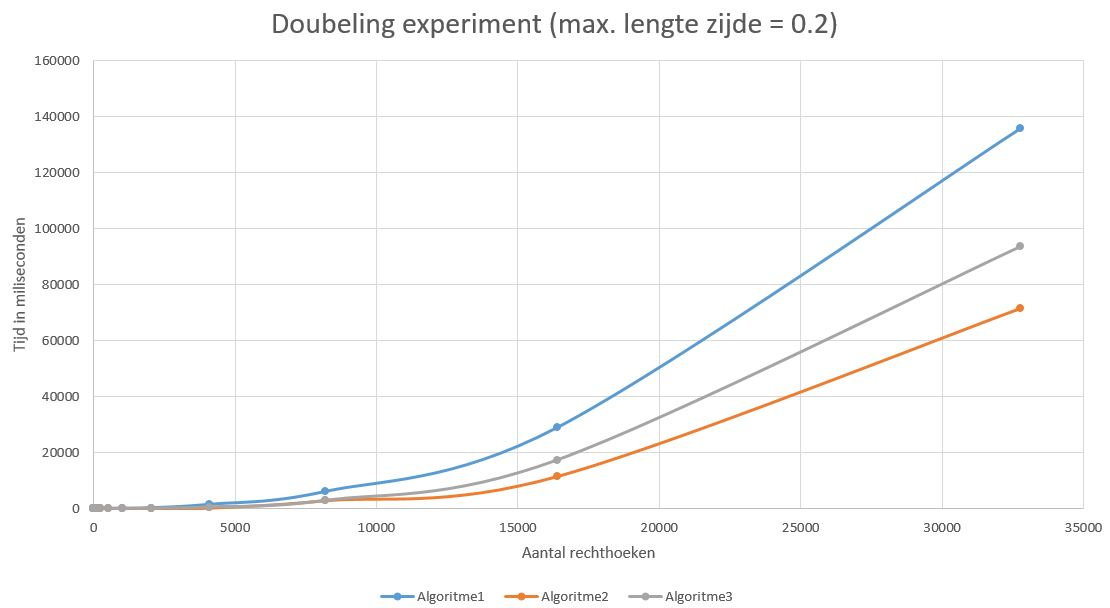
\includegraphics[width=0.75\textwidth]{zijde02.JPG}
				\caption{\label{fig:convR}Grafiek voor het doubeling experiment met zijdes die variëren tussen 0 en 0.2}
				\end{figure}
				\begin{figure}[H]
				\centering
				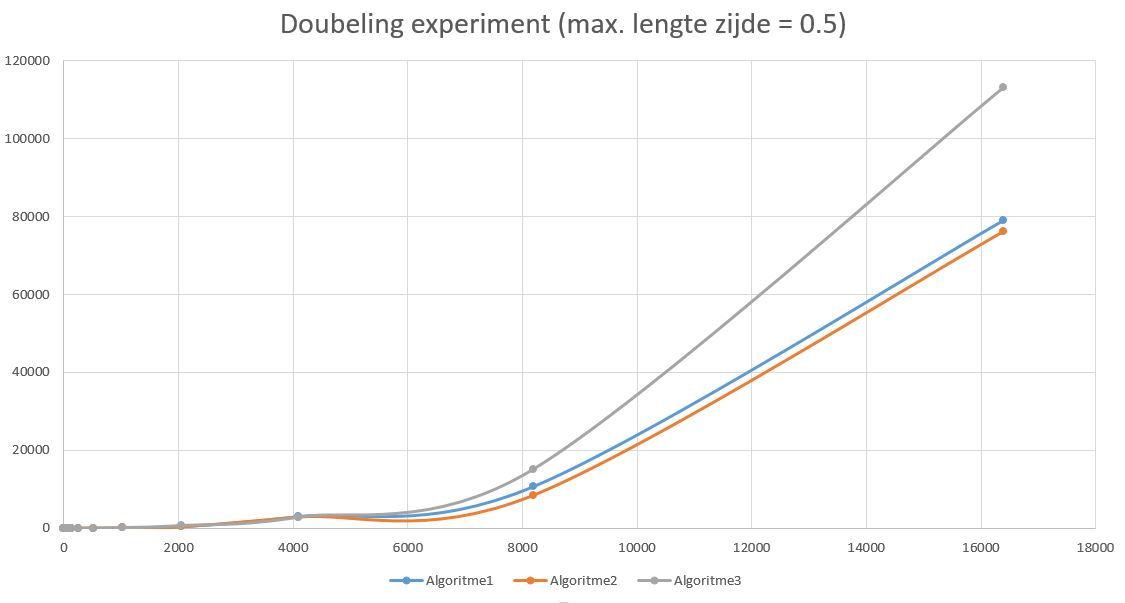
\includegraphics[width=0.75\textwidth]{zijde05.JPG}
				\caption{\label{fig:convR}Grafiek voor het doubeling experiment met zijdes die variëren tussen 0 en 0.5}
				\end{figure}
		\subsection{Correctheid}
			\subsubsection{Algoritme 1}
				Bij algoritme 1 vergelijken we elke rechthoek met elke andere rechthoek, zoals beschreven in vraag 1.  Alle rechthoeken worden dus met elkaar vergeleken voor snijpunten. Om te kijken of twee rechthoeken snijpunten hebben berekenen we eerst de overlappende rechthoek.  Als r1 en r2 twee rechthoeken zijn waarvan we de snijpunten willen vinden, dan bereken we de overlappende rechthoek (r3) met de volgende formule:
					$$r3.Lox = max(r1.Lox, r2.Lox)$$
					$$r3.Loy = max(r1.Loy, r2.Loy)$$
					$$r3.Rbx = min(r1.Rbx, r2.Rby)$$
					$$r3.Rby = min(r1.Rby, r2.Rby)$$
			De punten waar r1 en r2 mogelijk kunnen snijden zijn beperkt tot de vier hoekpunten van r3. Een hoekpunt van r3 kan alleen een snijpunt van r1 en r2 zijn als een van de volgende twee voorwaarden geldt:
				\begin{enumerate}
					\item Als de x-coördinaat van dat r3 hoekpunt een x-coördinaat is van een hoekpunt van r1 en wanneer dat de y-coördinaat van dat r3 hoekpunt een y-coördinaat is van een hoekpunt van r2.
					\item Als de x-coördinaat van dat r3 hoekpunt een x-coördinaat is van een hoekpunt van r2 en wanneer dat de y-coördinaat van dat r3 hoekpunt een y-coördinaat is van een hoekpunt van r1.
				\end{enumerate}
			Alle hoekpunten van r3 die aan deze voorwaarden voldoen zullen snijpunten zijn van de rechthoeken r1 en r2.  \\
			Om deze theorie nog eens te bevestigen hebben we onze resultaten ook nog eens grafisch gecontroleerd. We hebben een 50 tal keer de intersectie punten berekend voor een twintig tal willekeurig genereerde rechthoeken en de resultaten vervolgens grafisch gecontroleerd. Daarnaast hebben we zelf ook enkele randgevallen (zoals rechthoeken waarvan de zijdes samen vallen) bedacht en hiervan de intersectie punten berekend en vervolgens grafisch gecontroleerd. \\
			Aangezien dat onze theorie dus blijkt correct te zijn kunnen we dus veronderstellen dat algoritme 1 correct werkt.
			\subsubsection{Algoritme 2 en 3}
				Aangezien dat we er zeker van zijn dat algoritme 1 correct is hebben we dit ook gebruikt om de correctheid van algoritme 2 en 3 na te gaan.\\
				We hebben de computer in totaal 50 miljoen keer 20 willekeurige rechthoeken laten genereren en de intersectie punten hiervan laten bereken door de drie algoritme. Zowel algoritme 2 als 3 gaven dezelfde resultaten als algoritme 1. \\
				Daarnaast hebben we de computer ook een duizendtal keer 1500 willekeurige rechthoeken laten genereren en vervolgens de intersectie punten berekend met de drie algoritme. Ook voor deze test gaven de drie algoritme dezelfde resultaten.\\
				 Aangezien al deze testen waren geslaagd, kunnen we er vanuit gaan dat algoritme 2 en 3 ook correct werken.		
	\section{Bespreking resultaten}
		\subsection{Doubeling experiment met hoekpunten tussen 0 en 1}
			Wanneer we kijken naar de grafiek in figuur 1 dan zien we dat de tijd die de algoritmen nodig hebben steeds zeer snel stijgt. \\
			Voor het eerste algoritme zien we duidelijk dat dit kwadratisch blijkt te zijn, zoals we eerder hadden voorspeld.\\
			Voor het tweede algoritme lijkt ook bijna kwadratisch te zijn, maar toch iets sneller dan het eerste algoritme.  Dit komt omdat er zeer veel rechthoeken zijn waarvan de zijdes een lengte kunnen hebben die maximaal gelijk is aan de maximale x-coördinaat.  Met andere woorden er kunnen dus rechthoeken zijn die gedurende de volledige tijd dat het algoritme wordt uitgevoerd zich in de actieve lijst bevinden.  In het gemiddeld geval zal elke rechthoek dus een lengte hebben van 0.5.  Als we aannemen de rechthoeken uniform verspreid zijn, wil dit dus zeggen dat steeds de helft van het totale aantal rechthoeken zich in de actieve lijst bevindt. Hierdoor presteert algoritme 2 zeer slecht, bijna worst-case, omdat elke rechthoek wordt vergeleken met de helft van het totale aantal rechthoeken, dit is dus inderdaad geen geweldige verbetering t.o.v. algoritme 1.\\
			Algoritme 3 presteert nog het slechtst.  We hadden al eerder aangehaald dat het tweede algoritme in deze omstandig heden zeer slecht preseert, omdat er teveel elementen in de actieve lijst zitten. Algoritme 3 is bijna hetzelfde als algoritme 2  op het engie verschil na dat er gebruik wordt gemaakt van een Red-Black Tree voor het bijhouden van de actieve lijst.  Aangezien dat elke rechthoek twee keer wordt toegevoegd aan deze Red-Black Tree en dat het toevoegen van een element aan deze Red-Black Tree $\mathcal{O}(\log n)$ tijd kost, t.o.v. constante tijd voor het toevoegen van een element aan de een Array-list, is het dus niet moeilijk om in te zien dat dit algoritme in dit geval inderdaad slechter presteert. De kost van het bijhouden van een gesorteerde lijst met daarin alle actieve rechthoeken om zo onnuttige checks te vermijden (omdat andere rechthoeken in y-waarde zeer ver liggen van de desbetreffende rechthoek) is dus groter dan de kost om een rechthoek te vergelijken op snijpunten met alle andere actieve rechthoeken. Dit komt ook omdat de verticale zijdes van de rechthoeken zeer groot kunnen worden, waardoor de meeste rechthoeken in het actieve gebied elkaar toch zullen kruisen en het bijhouden van een gesorteerde lijst dus enkel meer tijd zal kosten en weinig voordeel zal bieden.
		\subsection{Doubeling experiment voor verschillende lengtes van de zijden}
			Zoals we zien op figuur 2, presteren algoritmes 2 en 3 veel beter wanneer de zijdes van de rechthoeken kleiner zijn.  We zien op deze grafiek duidelijk dat de tijscomplexiteit van algoritme 1 kwadratisch toeneemt, terwijl dat de algoritmen 2 en 3 zeer snel blijven. Dit komt omdat de lengte van zijden beperkt is tot 0.01 en de rechthoeken daardoor slechts kort in de actieve lijst blijven staan.  Op deze manier blijft het aantal rechthoeken waarmee een bepaalde rechthoek wordt vergeleken beperkt. Dit in tegenstelling met algoritme 1 waar elke rechthoek nog steeds wordt vergeleken met elke andere rechthoek ook al liggen die rechthoeken totaal niet in de buurt van elkaar. \\
			Omdat de lengte van zowel de horizontale als de verticale zijdes beperkt blijven tot 0.01, kan ook het aantal rechthoeken uit de actieve lijst waarmee snijpunten worden gezocht beperkt worden, dit omdat het aantal rechthoeken dat zich binnen de minimale en maximale y-coördinaat van de desbetreffende rechthoek bevindt, ook beperkt zal zijn. Daardoor zal algoritme 3 nu ook veel beter presteren.  Wanneer we kijken naar de resultaten in de tabel dan zien we duidelijk dat dit ook het geval is. De twee $\mathcal{O}(\log n)$ operaties die er nu moeten gebeuren om elke rechthoek in de actieve lijst te steken, wegen nu op tegen het aantal vergelijkingen dat er nu minder wordt gedaan. Dit kunnen we ook duidelijk zien in de onderstaande tabel. Naarmate het aantal rechthoeken toeneemt zal het derde algoritme steeds beter presteren t.o.v. het tweede omdat het een heleboel nutteloze berekeningen vermijdt.
		\begin{table}[H]
\centering
\begin{tabular}{ | l | l | l | l |}
\hline
\textbf{N}    &\textbf{Algoritme 1}  & \textbf{Algoritme 2} & \textbf{Algoritme 3} \\ \hline
1     & 0,055517    & 1,284362   & 1,282963  \\ \hline
2     & 0,076511    & 0,067647   & 0,059716 \\ \hline
4     & 0,059249    & 0,062981   & 0,16142   \\ \hline
8     & 0,165619    & 0,124564   & 0,202009    \\ \hline
16    & 0,793104    & 0,226734   & 0,501989    \\ \hline
32    & 1,287162    & 0,29065    & 0,74785     \\ \hline
64    & 4,109214    & 0,63635    & 1,774687     \\ \hline
128   & 9,296115    & 4,283696   & 2,997934     \\ \hline
256   & 24,111769   & 8,204431   & 4,207651    \\ \hline
512   & 45,772381   & 2,011219   & 4,963433   \\ \hline
1024  & 80,574263   & 3,626819   & 7,264368     \\ \hline
2048  & 205,435004  & 7,078222   & 12,793705   \\ \hline
4096  & 820,382407  & 11,974941  & 21,557508    \\ \hline
8192  & 3289,07998  & 31,238512  & 24,914204   \\ \hline
16384 & 15940,14955 & 102,42475  & 65,278081    \\ \hline
32768 & 67381,76355 & 460,93495  & 225,83225    \\ \hline
65536 & 285255,7015 & 1555,7538  & 747,09444 \\ \hline
\end{tabular}
\caption{Tijd in miliseconden die elk algoritme nodig heeft om de snijpunten van rechthoeken met maximale zijden van 0.01 te berekenen.}
\end{table}
Aan figuur 3 tot 5 zien we duidelijk dat algoritmes 2 en 3 duidelijk slechter gaan presteren naarmate de lengte van de zijden toeneemt.  Zoals eerder al uitgelegd komt dit omdat de actieve lijst steeds groter wordt en er dus steeds meer rechthoeken met elkaar worden vergeleken. Dat algoritme 3 uiteindelijk slechter presteert dan algoritme 2 is omdat het de kost voor het geordend houden van de actieve lijst niet opweegt tegen het aantal vergelijkingen dat wordt vermeden, dit wederom omdat naarmate de zijden groter worden de rechthoeken ook steeds meer en meer in de y-richting op elkaar gaan liggen en het dus uiteindelijk gemakkelijker wordt om alle rechthoeken met elkaar te vergelijken op snijpunten, dan het bijhouden van de geordende lijst waaruit uiteindelijk toch bijna alle rechthoeken moeten worden gehaald.  Bij algoritme 3 moet het controleren op snijpunten met andere rechthoeken ook nog eens twee keer gebeuren, één keer bij het toevoegen van de rechthoek aan de actieve lijst en één keer bij het verwijderen.
	
\end{document}